% Packages
\documentclass[12pt]{article}
\usepackage[margin=2.5cm]{geometry}
\usepackage{lipsum}
\usepackage{titlesec, titletoc}
\usepackage[svgnames, table]{xcolor}
\usepackage{algorithm}
\usepackage{algpseudocode}
\usepackage{mdframed}
\usepackage[T1]{fontenc}
\usepackage{amsmath,amsthm,amsfonts,amssymb,mathtools}
\usepackage[osf]{mathpazo}
\usepackage{enumitem}

% Formating setup
\footskip = 1 cm
\setlength{\parindent}{0pt}
\pdfpxdimen=1in
\parindent = 0pt
\definecolor{myBlue}{RGB}{0, 81, 255}
\titleformat{\section}[block]{\sffamily\large\bfseries}{\thesection}{.5em}{\textcolor{myBlue}
{\titlerule[1.5pt]}\\\sffamily}[\vspace*{-3mm}\textcolor{myBlue}{\titlerule[1.5pt]}]
\titleformat{\subsection}{\large\sffamily\bfseries}{\thesubsection}{0.5em}{\textcolor{Black}}
\newcounter{boxedlistcounter}
\newenvironment{pseudo}{%
  \setcounter{boxedlistcounter}{0}% <-- Add this line to reset the counter
  \mdframed[
    linecolor=black, % color of the border
    linewidth=1.5pt, % thickness of the border
    roundcorner=10pt, % radius of the corners
    innertopmargin=0.6\baselineskip, % space at the top of the box
    innerbottommargin=0.6\baselineskip, % space at the bottom of the box
  ]
  \fontsize{12pt}{14pt}\selectfont % add font size command here
  \mdseries % add font series command here
}{%
  \endmdframed%
}
\newcommand{\I}{\par\stepcounter{boxedlistcounter}\arabic{boxedlistcounter}.\hspace{5pt}}
\newcounter{boxedlistcounter2}
\newenvironment{Proof}{%
  \refstepcounter{boxedlistcounter2}%
  \mdframed[
    linecolor=black, % color of the border
    linewidth=1.5pt, % thickness of the border
    roundcorner=10pt, % radius of the corners
    innertopmargin=\baselineskip, % space at the top of the box
    innerbottommargin=\baselineskip, % space at the bottom of the box
  ]
  \fontsize{12pt}{14pt}\selectfont % add font size command here
  \mdseries % add font series command here
}{%
  \endmdframed%
}
\newcommand{\PI}{\par\textbullet\hspace{5pt}}
\setlist[itemize]{itemsep=1pt}
\newcommand{\NL}{\par\hspace{12.5pt}}
\setlist[itemize]{itemsep=1pt}

% Custom commands
\newcommand{\for}[1]{\textbf{for} #1 \textbf{do}}
\newcommand{\IF}[1]{\textbf{if} #1 \textbf{then}}
\newcommand{\ELIF}[1]{\textbf{else if} #1 \textbf{then}}
\newcommand{\ELSE}{\textbf{else}}
\newcommand{\return}[1]{\textbf{return} #1}
\newcommand{\assign}{ $\leftarrow$ }
\newcommand{\DEF}[2]{\textbf{def} #1(#2):}
\newcommand{\1}{\space \quad}
\newcommand{\2}{\quad \quad \quad}
\newcommand{\3}{\quad \quad \quad \quad \space}
\newcommand{\4}{\quad \quad \quad \quad \quad \quad}
\newcommand{\comment}[1]{\hfill \textit{\# #1}}

% Document start ------------------------------------------------------------------------------------
\begin{document}

% Section 1  ----------------------------------------------------------------------------------------
\section{Introduction to trees}
A tree T is made up of a set of nodes endowed with parent-child relationship with following properties:
\begin{itemize}
  \item If T is non-empty, it has a special node called the root that has no parent
  \item Every node v of T other than the root has a unique parent
  \item Following the parent relation always leads to the root (i.e., the parent-child relation does not have 
  “cycles”)
\end{itemize}

\subsection{Terminology}
\begin{itemize}
  \item Root: node without parent.
  \item Internal node: node with at least one child.
  \item External/leaf node: node without children.
  \item Ancestors: parent, grandparent, great-grandparent, etc.
  \item Descendants: child, grandchild, great-grandchild, etc.
  \item Two nodes with the same parent are siblings. 
  \item Depth of a node: number of ancestors not including itself.
  \item Level: set of nodes with given depth.
  \item Height of a tree: maximum depth.
  \item Subtree: tree made up of some node and its descendants. 
  \item Edge: a pair of nodes (u, v) such that one is the parent of the other.
  \item Path: sequence of nodes such that consecutive nodes in the sequence have an edge
\end{itemize}
\textbf{Tree facts}
\begin{itemize}
  \item If node X is an ancestor of node Y, then Y is a descendant of X.
  \item Ancestor/descendant relations are transitive.
  \item Every node is a descendant of the root.
  \item There may be nodes where neither is an ancestor of the other.
  \item Every pair of nodes has at least one common ancestor. 
  \item The lowest common ancestor (LCA) of x and y is a node z such that z is the ancestor of x and y and no descendant of z has that property.
  \item In an ordered tree there is a prescribed order for each node’s children.
\end{itemize}

% Section 2  ----------------------------------------------------------------------------------------
\section{Traversal}
\subsection{Preorder Traversal}
To do a preorder traversal starting at a given node, we visit the node before visiting its descendants
If tree is ordered visit the child subtrees in the prescribed order. Visit does some work on the node such
as print node data, aggregate node data or modify node data. The example shows a pre\_order traversal called at
root.
\begin{pseudo}
  \I \DEF{pre\_order}{v}
  \I \1 visit(v)
  \I \1 \for{each child w of v}
  \I \2 pre\_order(w)
\end{pseudo}
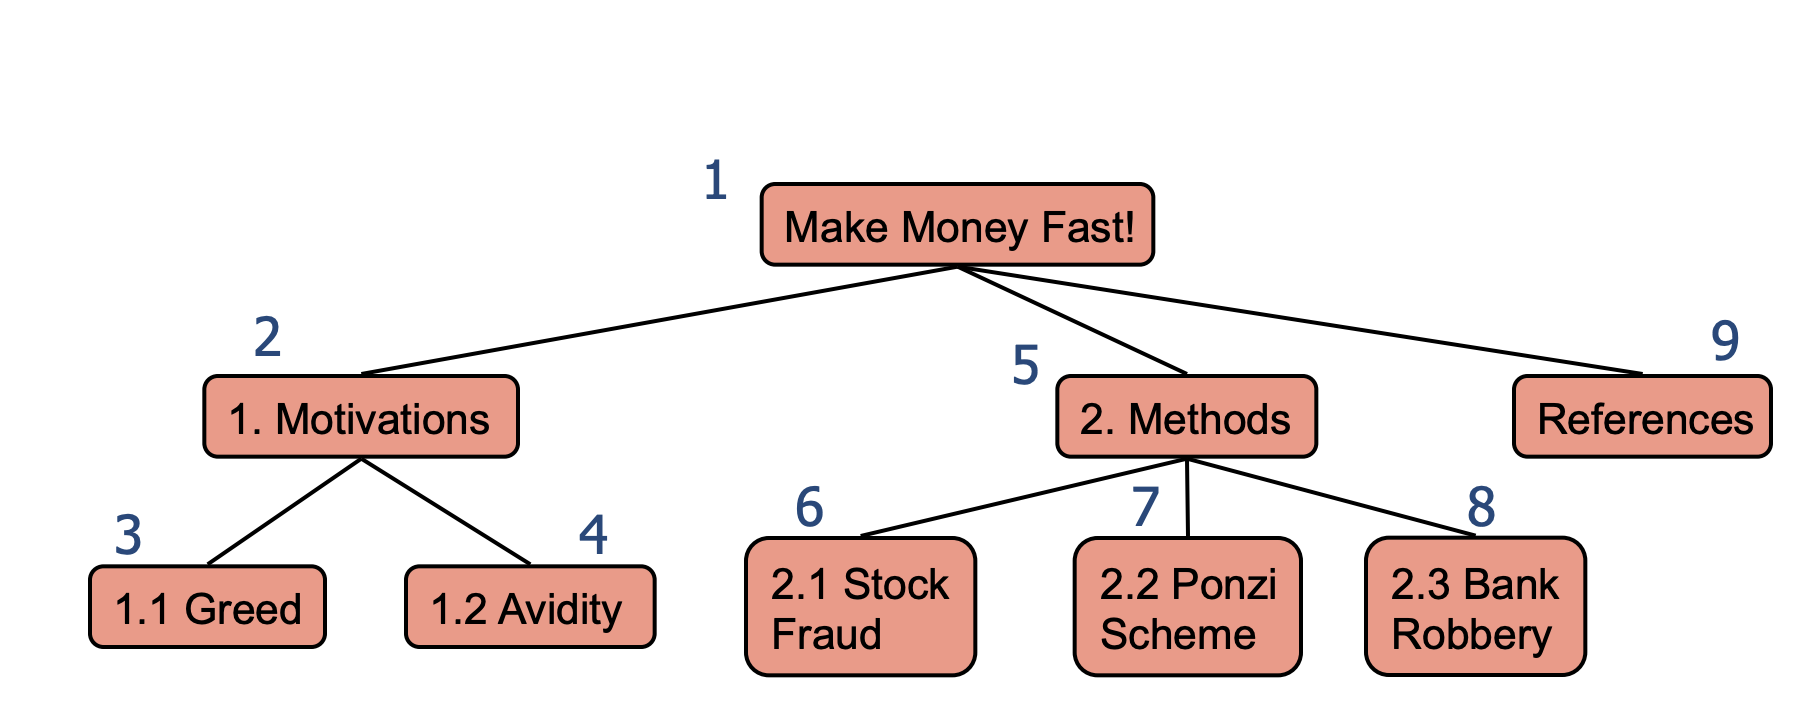
\includegraphics[width=\textwidth]{image1.png}

\subsection{Postorder Traversal}
To do a postorder traversal starting at a given node, we visit the node after its descendants
If tree is ordered visit the child subtrees in the prescribed order.
\begin{pseudo}
  \I \DEF{pre\_order}{v}
  \I \1 \for{each child w of v}
  \I \2 pre\_order(w)
  \I \1 visit(v)
\end{pseudo}
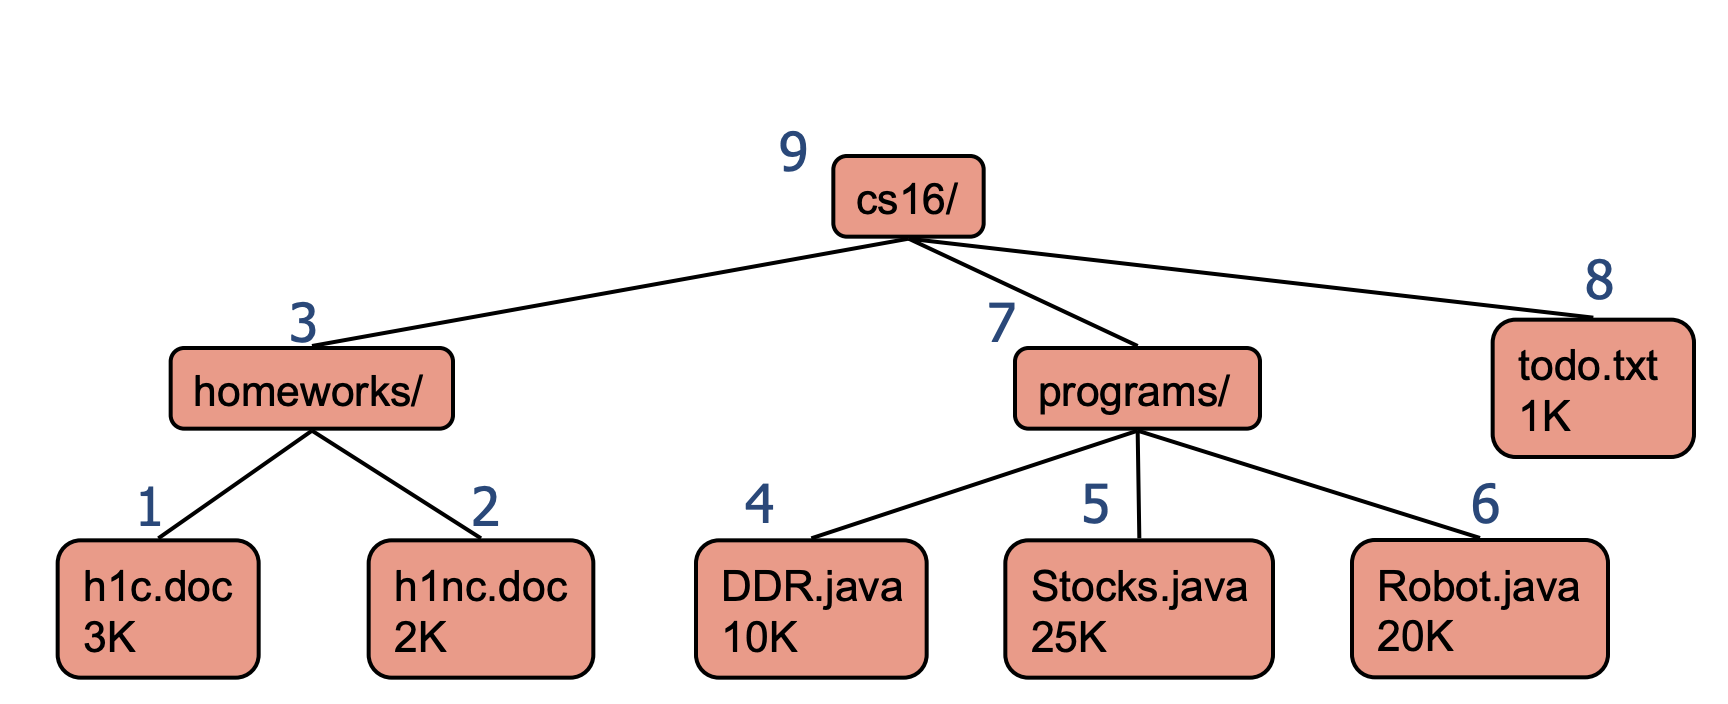
\includegraphics[width=\textwidth]{image2.png}

% Section 3  ----------------------------------------------------------------------------------------
\section{Binary Trees}
A binary tree is an ordered tree with the following properties: Each internal node has at most two children.
Each child node is labeled as a left child or a right child. Child ordering is left followed by right.
The right/left subtree is the subtree root at the right/left child. We say the tree is proper if every
internal node has two children.
\begin{pseudo}
  \I \DEF{is\_external}{v} \comment{Tests if v is a leaf}
  \I \1 \return{v.left = null and v.right = null}
\end{pseudo}

\subsection{Inorder Traversal}
To do an inorder traversal starting at a given node, the node is visited after its left subtree 
but before its right subtree.

\begin{minipage}[l]{0.6\textwidth}
  \begin{pseudo}
    \I \DEF{in\_order}{v}
    \I \1 \IF{v.left != null}
    \I \2 in\_order(v.left)
    \I \1 visit(v)
    \I \1 \IF{v.right != null}
    \I \2 in\_order(v.right)
  \end{pseudo}
\end{minipage}
\begin{minipage}[r]{0.39\textwidth}
  \raggedleft
  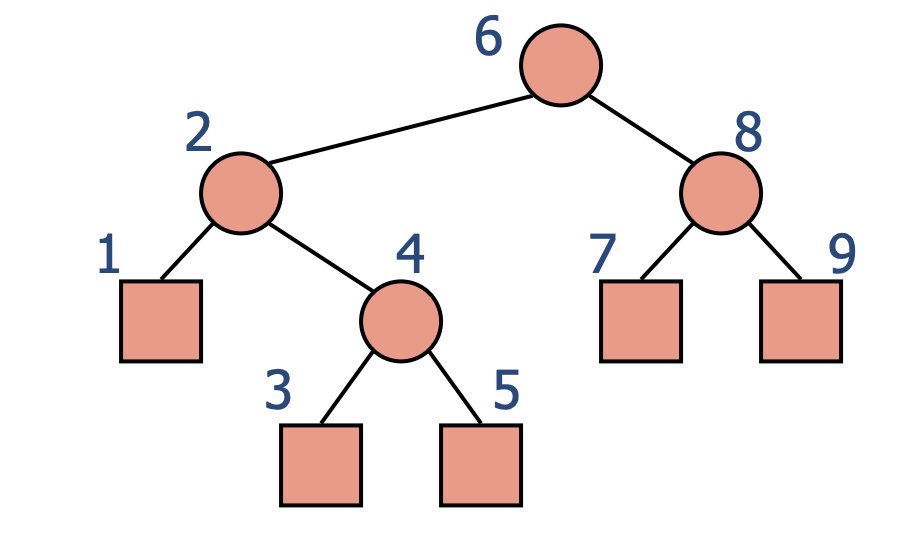
\includegraphics[width=\textwidth]{image3.png}
\end{minipage}

% Section 4  ----------------------------------------------------------------------------------------
\section{Euler Tour Traversal \& Some code}
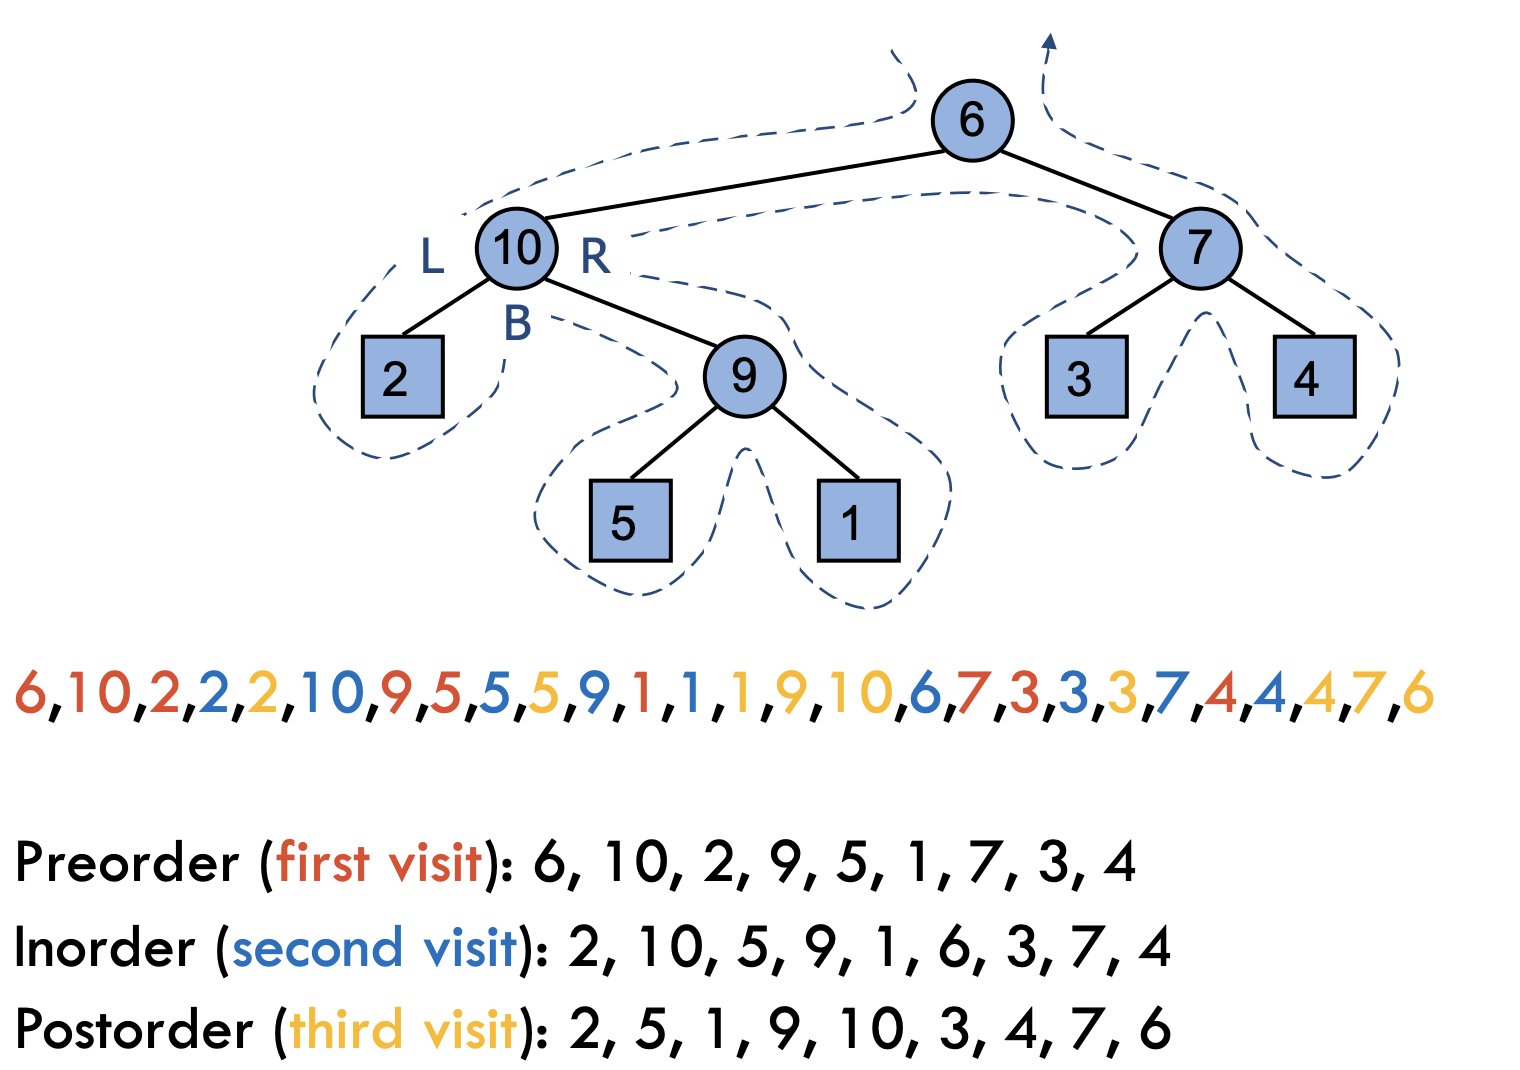
\includegraphics[width=0.90\textwidth]{image4.png}
\vspace{20pt}
\begin{pseudo}
  \I \DEF{height}{v} \comment{compute height of subtree at v}
  \I \1 \IF{v.parent = null} \comment{root’s depth is 0}
  \I \2 \return{$0$}
  \I \1 \ELSE
  \I \2 \return{depth(v.parent) + 1}
\end{pseudo}
\begin{pseudo}
  \I \DEF{depth}{v} \comment{compute height of subtree at v}
  \I \1 \IF{v.isExternal()} \comment{a leave’s height is $0$}
  \I \2 \return{$0$}
  \I \1 \ELSE{}
  \I \2 h \assign $0$
  \I \2 \for{each child w of v}
  \I \3 h \assign max(h, height(w))
  \I \2 \return{h + 1}
\end{pseudo}

% Section 5  ----------------------------------------------------------------------------------------
\section{Binary Search Trees}
A binary search tree is a binary tree storing keys (or key-value pairs) satisfying the following BST property.
\textbf{"For any node v in the tree and any node u in the left subtree of v and any node w in the right subtree of v,
key(u) < key(v) < key(w)"}

\subsection{BST Implementation}
To simplify BST implementation, keys (or key-value pairs) are only stored in internal noves and not extreenal nodes,
with external nodes being null.
To search for a key k, we trace a downward path starting at the root. To decide whether to go left or right,
we compare the key of the current node v with k. If we reach an external node, this means that the key is not 
in the data structure.
\begin{pseudo}
  \I \DEF{search}{k, v}
  \I \1 \IF{v.isExternal()}
  \I \2 \return{v} \comment{unsuccessful search}
  \I \1 \IF{k = v.key()}
  \I \2 \return{v} \comment{successful search}
  \I \1 \IF{k < v.key()}
  \I \2 \return{search(k, v.left)}
  \I \1 \ELSE \comment{k > v.key()}
  \I \2 \return{search(k, v.right)}
\end{pseudo}
Runs in O(h) time, where h is the height of the tree. In the wort case h = n-1 and in the best case, $h <= log_2n$

To perform operation put(k, 0), we search for key k (using search). If k is found in the tree, replace the corresponding
value by o. If k is not found, let w be the external node reached by the seached by the search. We replace w with an
internal node storing key k and value o and two external nodes as children. The new node is a leaf and the tree is
proper. The operation put runs in O(h) time.

To perform operation remove(k), we search for key k (using search) to find the node w holding k. We distinguish between two cases
being, w has one external child and w having two internal children. If k is not in the tree, we can either throw an exception or do
nothing depending on the ADT specs.

\begin{itemize}
  \item \textbf{Deletion Case 1}: Suppose that the node w we want to remove has an external child, which
  we call z. To remove w we remove w and z from the tree. We then promote the other child of w to take w's place.
  This preserves the BST property.
  \item \textbf{Deletion Case 2}: Suppose that the node w we want to remove has two internal children. To remove w,
  we find the internal node y following w in an inorder traversal (i.e., y has the smallest key among the right subtree under w).
  we copy the entry from y into node w. we remove node y and its left child z, whcih must be external. This preserves the BST property.
\end{itemize}

\begin{pseudo}
  \I \DEF{remove}{k}
  \I \1 w \assign search(k, root)
  \I \1 \IF{w.isExternal()}
  \I \2 \return{null} \comment{key not found}
  \I \1 \ELIF{w has at least one external child z}
  \I \2 remove z
  \I \2 promote the other hcild of w to take w's place
  \I \2 remove w
  \I \1 \ELSE \comment{w has two internal children}
  \I \2 y \assign w's successor in an inorder traversal
  \I \2 replace contents of w with entry from y
  \I \2 remove y as above
\end{pseudo}

\textbf{Complexity}
Consider a binary search tree with n items and height h. The sapce used is O(n) and get, put and remove take O(h). The height h can be n in the
worst case and log(n) in the best case. Therefore, using better insertion routines can drastically cut running times.

\subsection{Duplicate key values in BST}
It is possible to allow duplicates, but it comes at the cost of additional compleixty.
\begin{itemize}
  \item Allowing left descendants to be equal to the parent. i.e. $key(left descendant) <= key(node) <= key(right descendant)$ 
  \item Using a list to store duplicates.
\end{itemize}

\subsection{Range Queries}
A range querey is defined by two values $k_1$ and $k_2$. We are to find all ekys k stored in T such that $k_1 <= k <= k_2$.
The algorithm is a restricted version of inorder traversal. When at node v:
\begin{itemize}
  \item If $key(v) < k_1$: Recursively search right subtree
  \item If $k_1 <= key(v) <= k_2$: Recursively search left subtree, add v to range output, search right subtree.
  \item If $k_2 < key(v)$: REcursively search left subtree
\end{itemize}

\begin{pseudo}
  \I \DEF{range\_search}{T, k1, k2}
  \I \1 output \assign []
  \I \1 range(T.root, k1, k2)
\end{pseudo}

\begin{pseudo}
  \I \DEF{range}{v, k1, k2}
  \I \1 \IF{v is external}
  \I \2 \return{null}
  \I \1 \IF{key(v) > k2}
  \I \2 range(v.right, k1, k2)
  \I \1 \ELIF{key(v) < k1}
  \I \2 range(v.right, k1, k2)
  \I \1 \ELSE
  \I \2 \hspace{1.1pt} range(v.left, k1, k2)
  \I \2 output.append(v)
  \I \2 range(v.right, k1, k2)
\end{pseudo}
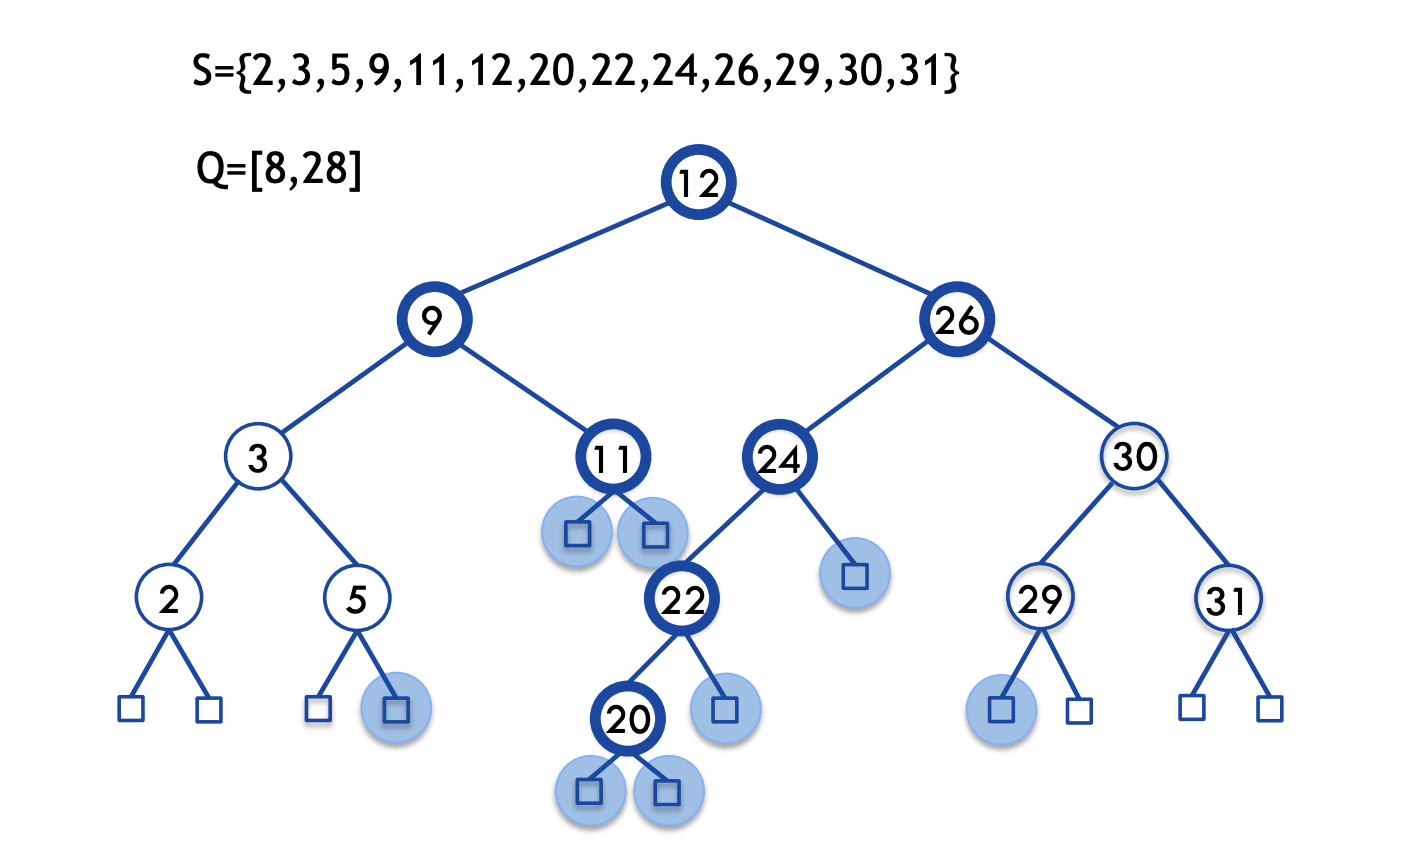
\includegraphics[width=\textwidth]{image5.png}

\textbf{Performance}
Let $P_1$ and $P_2$ be the binary search paths to $k_1$ and $k_2$. We say a node v is a:
\begin{itemize}
  \item Boundary node if v in $P_1$ or $P_2$
  \item Inside node if key(v) in [$k_1$, $k_2$] but not in $P_1$ or $P_2$
  \item Outside node if key(v) not in [$k_1$, $k_2$] and not in $P_1$ or $P_2$
\end{itemize}

The alogirithm only vists boundary and inside nodes and $|inside nodes| <= |output|$ and
$|boundary nodes| <= 2 * tree height$. Therefore, since we only spend O(1) time per node 
we visit, the total running time of range search is O($|output| + tree height$)

% Section 6  ----------------------------------------------------------------------------------------
\section{Maintaining a balanced BST}
Ranked balanced trees are a family of balanced BST implementations that use the idea of
keeping a “rank” for every node, where r(v) acts as a proxy measure of the size of the 
subtree rooted at v. This is primarily done to reduce the discrepancy between the ranks of
left and right subtrees.

\subsection{AVL trees}
AVL trees are rank-balanced trees, where r(v) is its height of the subtree rooted at v.
Balance constraint: The ranks of the two children of every internal-node differ by at most 1

\vspace{10pt}
\textbf{Proof (by induction)}: The height of an AVL tree stroing n keys is O(logn)
\begin{Proof}
  \PI Let N(h) be the minimum number of keys of an AVL tree of height h.
  \PI We can easily see that N(1) = 1 and N(2) = 2
  \PI Clearly N(h) > N(h-1) for any h >= 2.
  \PI For For h > 2, the smallest AVL tree of height h contains the root node, one AVL 
  \NL subtree of height h-1 and another of height at least h-2:
  \PI N(h) >= 1 + N(h-1) + N(h-2) > 2 N(h-2)
  \PI By induction we can show that for h even N(h) >= $2^{h/2} $
  \PI Taking logarithms: h < 2 log N(h)
  \PI Thus the height of an AVL tree is O(log n)
\end{Proof}

\subsection{Insertion in AVL trees}
Suppose we are to insert a key k into our tree:
\begin{itemize}
  \item If k is in the tree, search for k ends at node holding k. There is nothing to do so tree structure does not change
  \item If k is not in the tree, search for k ends at external node w. Make this be a new internal node containing key k
  \item The new tree has BST property, but it may not have AVL balance property at some ancestor of w since some ancestors 
  of w may have increased their height by 1 and every node that is not an ancestor of w hasn’t changed its height.
  \item We use rotations to re-arrange tree to re-establish AVL property, while keeping BST property.
\end{itemize}

% Section 7  ----------------------------------------------------------------------------------------
\newpage
\section{Re-establishing AVL property}
\begin{itemize}
  \item Let w be the location of a newly inserted node. (54)
  \item Let z be the lowest ancestor of w, whose children heights differ by 2.
  \item Let y be the child of z that is the ancestor of w.
  \item Let x be the child of y that is is the ancestor of w.
\end{itemize}
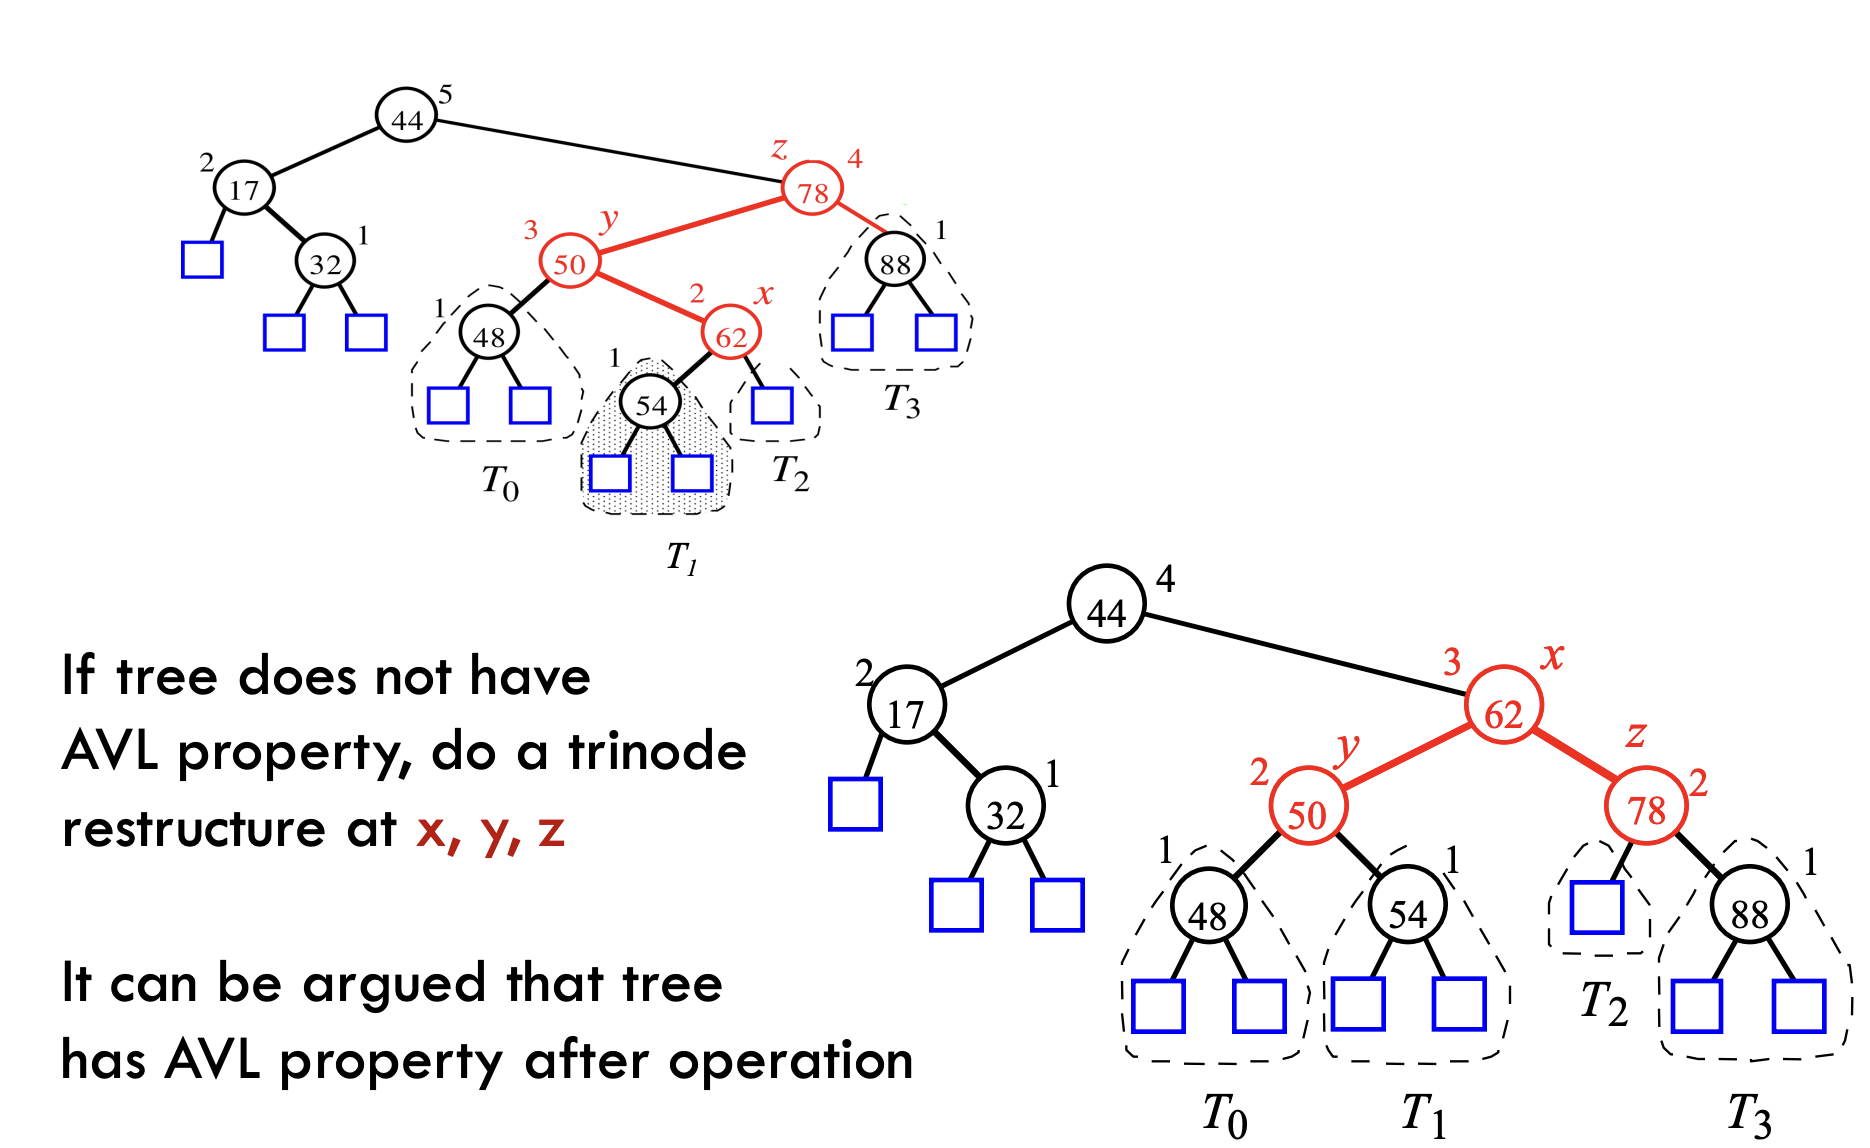
\includegraphics[width=\textwidth]{image6.png}

\subsection{Augmenting BST with a height attribute}
But how do we know the height of each node? If we had to compute this from scratch it would take O(n) time
Therefore, we need to have this pre-computed and update the height value after each insertion and rebalancing operation:
After we create a node w, we should set its height to be 1, and then update the height of its ancestors. After we rotate 
(z, y, x) we should update their height and that of their ancestors. Thus, we can maintain the height only using O(h) work 
per insert

\newpage
\begin{pseudo}
  \I \DEF{reststructure}{x} \comment{O{1}}
  \NL \textbf{Input:} A node x of a binary tree T that has boath a parent y and a grandparent z.
  \NL \textbf{Output:} The tree T after a trinode restrcucting (single or double roation)
  \I  Let (a,b,c) be the left-to-right (inorder) listing of the nodes x, y, and z, and let 
  \NL (T0,T1,T2,T3) be the left-to-right (inorder) listing of the four subtrees of x, y, and z 
  \NL that are not rooted at x, y, and z. 
  \I  Replace the subtree with a new subtree rooted at b.
  \I  Let a be the left child of b and let T0 and T1 be the left and right subtrees of a.
  \I  Let c be the right child of b and let T2 and T3 be the left and right subtrees of c.
  \I  Recalculate the heights of a, b, and c from the values stored at their children
  \I  \return{b}
\end{pseudo}

\begin{center}
  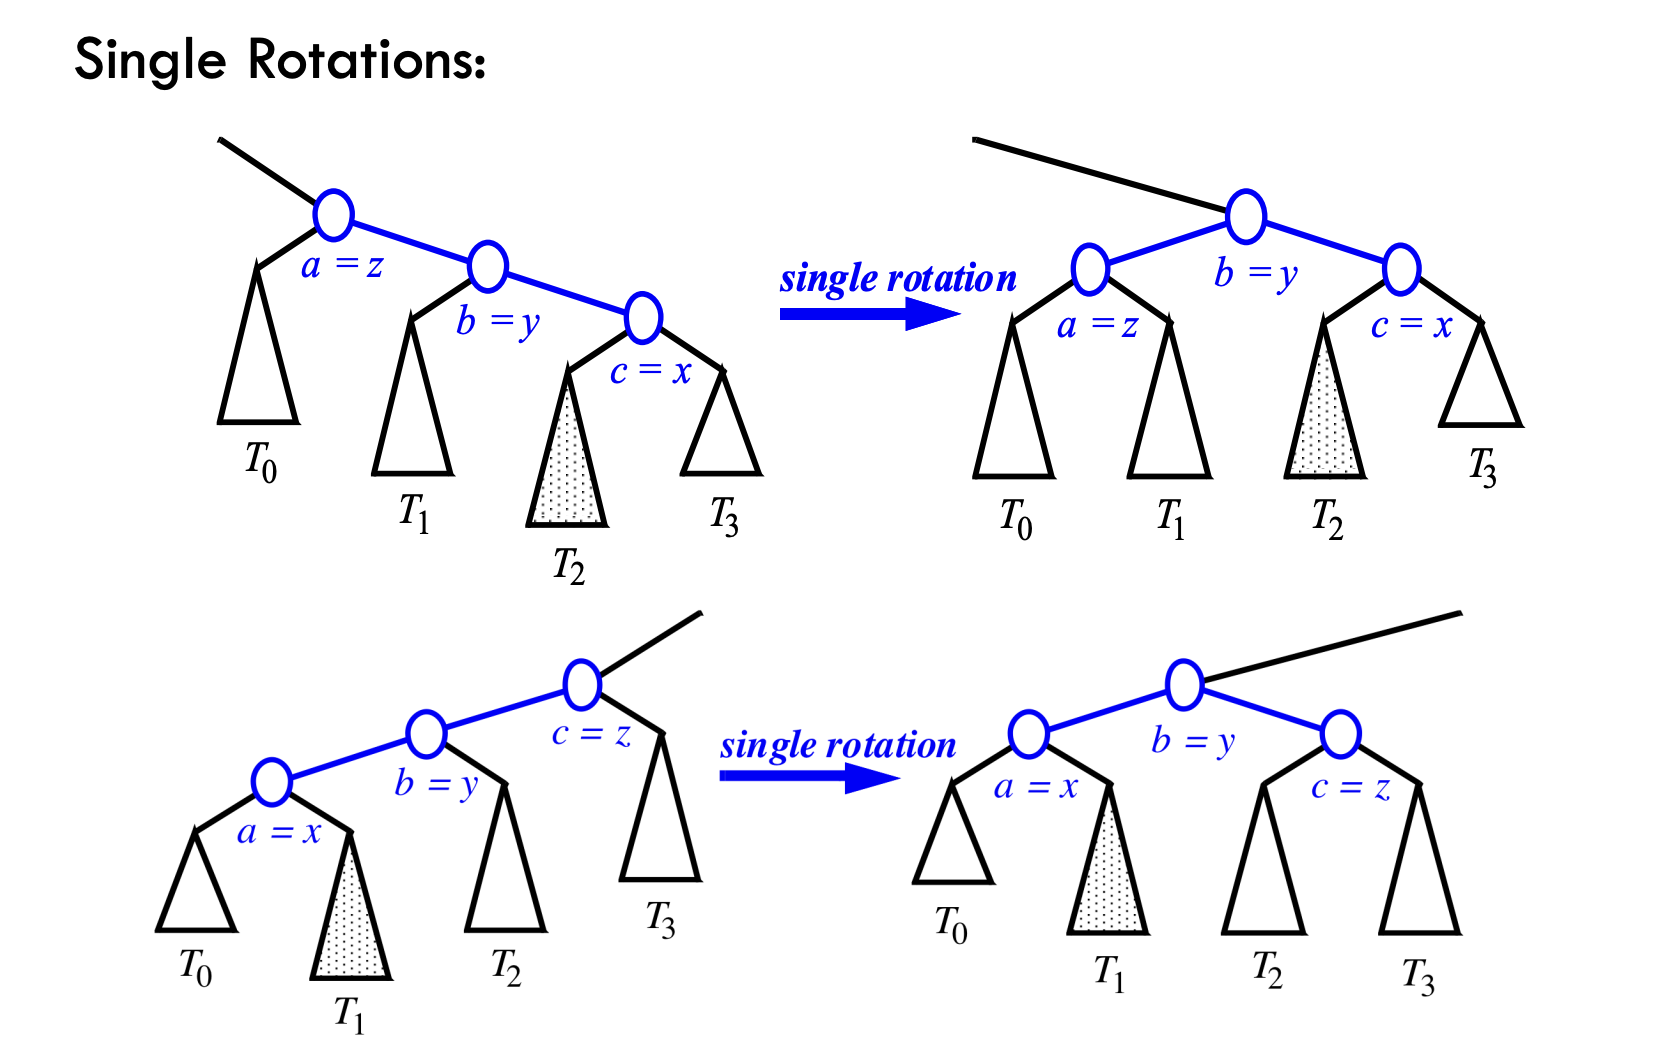
\includegraphics[width=0.75\textwidth]{image7.png}
  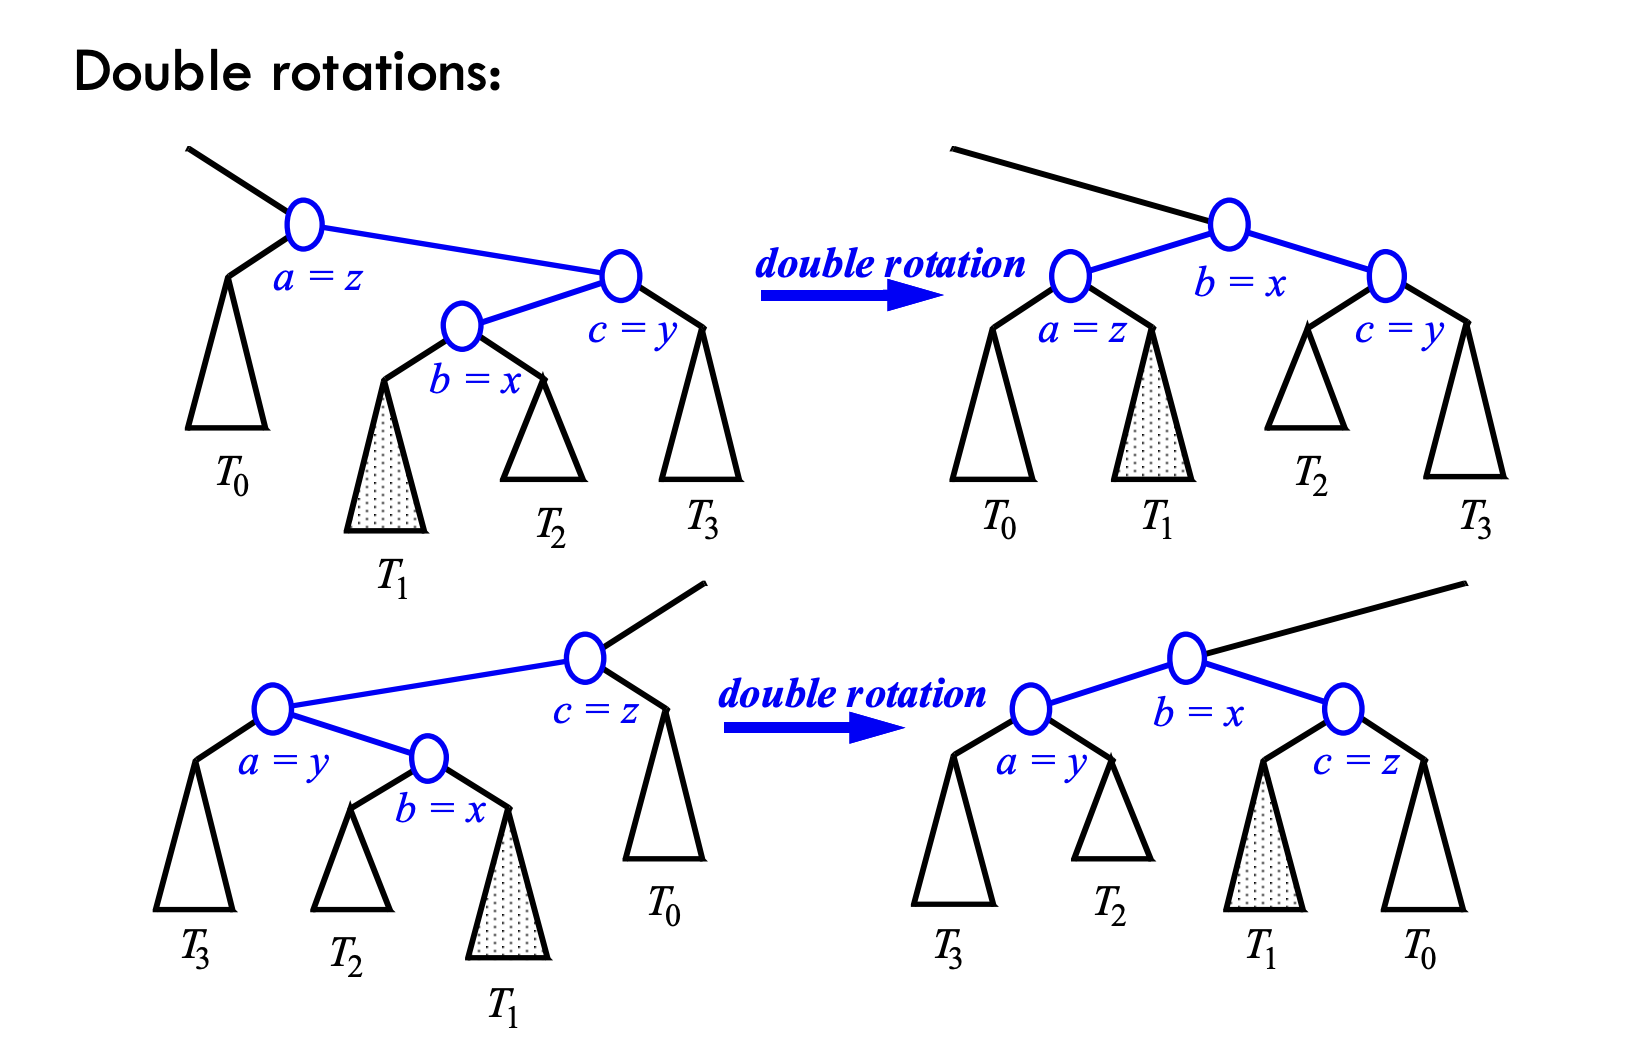
\includegraphics[width=0.75\textwidth]{image8.png}
\end{center}

\subsection{Removal in AVL trees}
\textbf{Suppose we are to remove a key k from our tree:}
\begin{itemize}
  \item If k is not in the tree, search for k ends at external node. There is nothing to do so tree structure does not change.
  \item If k is in the tree, search for k performs usual BST removal leading to removing a node with an external child and promoting its other child, which we call w.
  \item The new tree has BST property, but it may not have AVL balance property at some ancestor of w since some ancestors of w may have decreased their height by 1 and every node that is not an ancestor of w hasn’t changed its heights.
  \item We use rotations to rearrange tree and re-establish AVL property, while keeping BST property.
\end{itemize}
\textbf{Re-establishing AVL property}
\begin{itemize}
  \item Let w be the parent of deleted node.
  \item Let z be the lowest ancestor of w, whose children heights differ by 2.
  \item Let y be the child of z with larger height (y is not an ancestor of w).
  \item Let x be child of y with larger height.
\end{itemize}
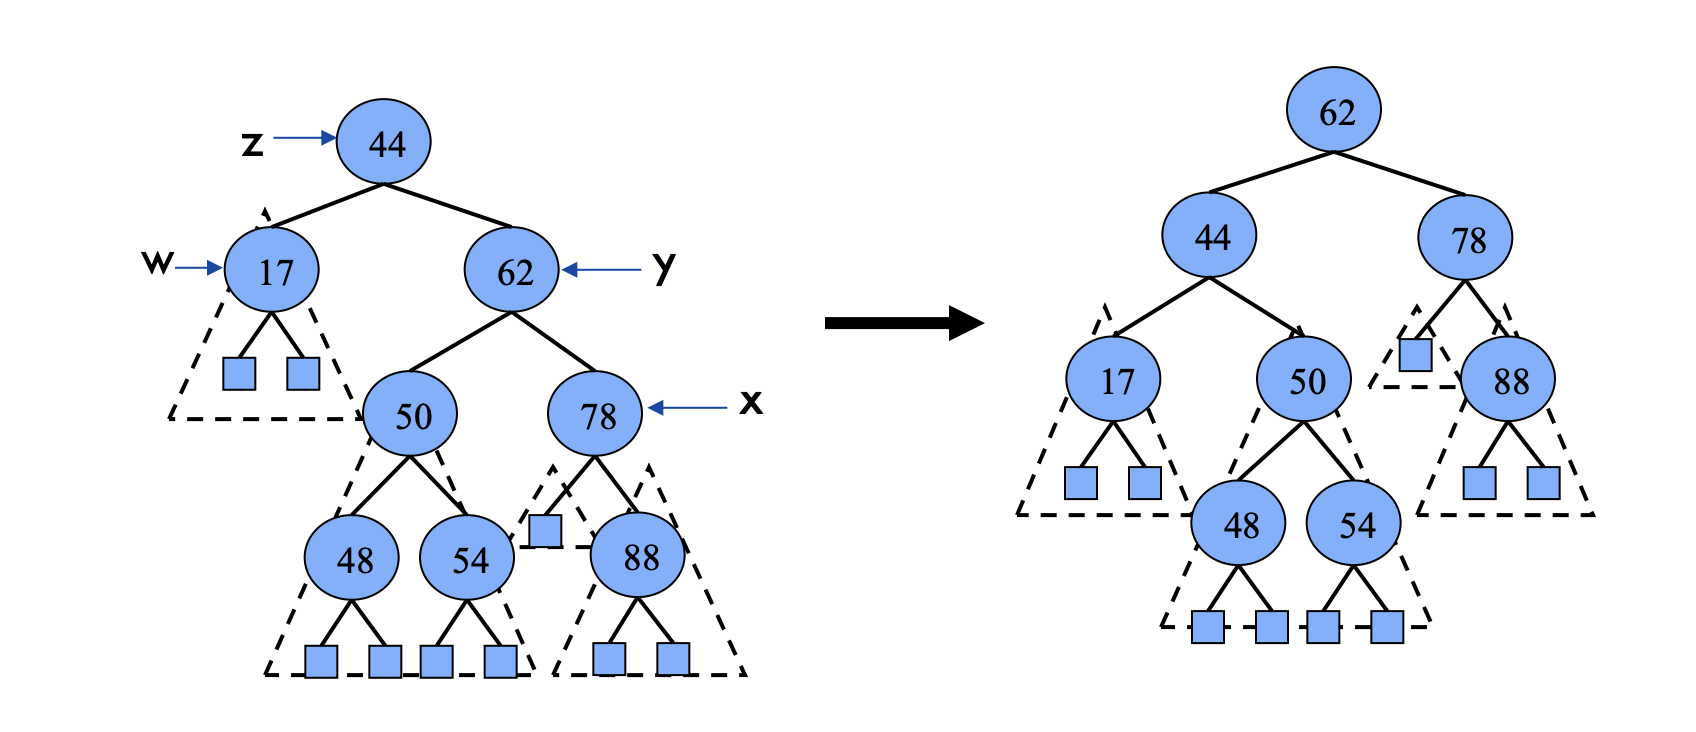
\includegraphics[width=\textwidth]{image9.png}
This restores the AVL property at z, but it may upset the balance of another node higher in the tree, we must continue checking for balance until the root of T is reached.

\subsection{AVL Tree Performance}
The data structure uses O(n) space. Height of the tree O(log n). Searching takes O(log n) time. Insertion takes O(log n) time. Removal takes O(log n) time
\end{document}